\documentclass[hyperref={unicode}]{beamer}
%
% Choose how your presentation looks.
%
% For more themes, color themes and font themes, see:
% http://deic.uab.es/~iblanes/beamer_gallery/index_by_theme.html
%
\mode<presentation> {
	\usetheme{Berkeley}      % or try Darmstadt, Madrid, Warsaw, ...
	\usecolortheme{seahorse} % or try albatross, beaver, crane, ...
	\usefonttheme{default}  % or try serif, structurebold, ...
	\setbeamertemplate{navigation symbols}{}
%	\setbeamertemplate{caption}[numbered]
	\setbeamertemplate{caption}{\raggedright\insertcaption\par}		
	% Numbered bibiolgraphy items
%	\setbeamertemplate{bibliography item}{\insertbiblabel}
} 

\usepackage[utf8]{inputenc}
\usepackage[english]{babel}
\usepackage[T1]{fontenc}
\usepackage{csquotes,lmodern,silence}
%\usepackage[style=numeric,backend=biber]{biblatex}

%\WarningFilter{biblatex}{Patching footnotes failed}

% Remove small caps warning
%\renewcommand\mkbibacro[1]{{\footnotesize\MakeUppercase{#1}}}

%\addbibresource{bibliography.bib}
\graphicspath{{figures/}}

\title[Linux Boards]{Linux Boards}
\author{Peter Babič}
\institute{Technical University of Košice, Slovakia}
\date{21.05.2015}

\begin{document}

\begin{frame}
  \titlepage
\end{frame}

%\begin{frame}{Talk Outline}
%  \tableofcontents
%\end{frame}



\section{Introduction}

\begin{frame}{Introduction}
	What is a Linux Board? Where did it come from?
	\begin{figure}
	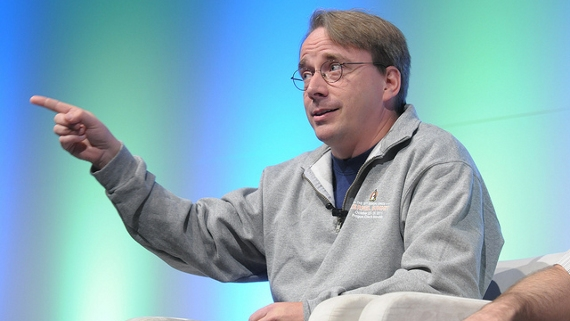
\includegraphics[width=.7\textwidth]{linus-torvalds-linuxcon.jpg}
	\caption{I don't have time for this!}
	\end{figure}
\end{frame}


\section{Boards}

%\begin{frame}{Board Categorization}
%\begin{itemize}
%\item Single Board Computer
%\item Embedded module
%\item Development board
%\end{itemize}
%\end{frame}



\subsection{Single Board Computers}

\begin{frame}{Single Board Computer}
\begin{figure}
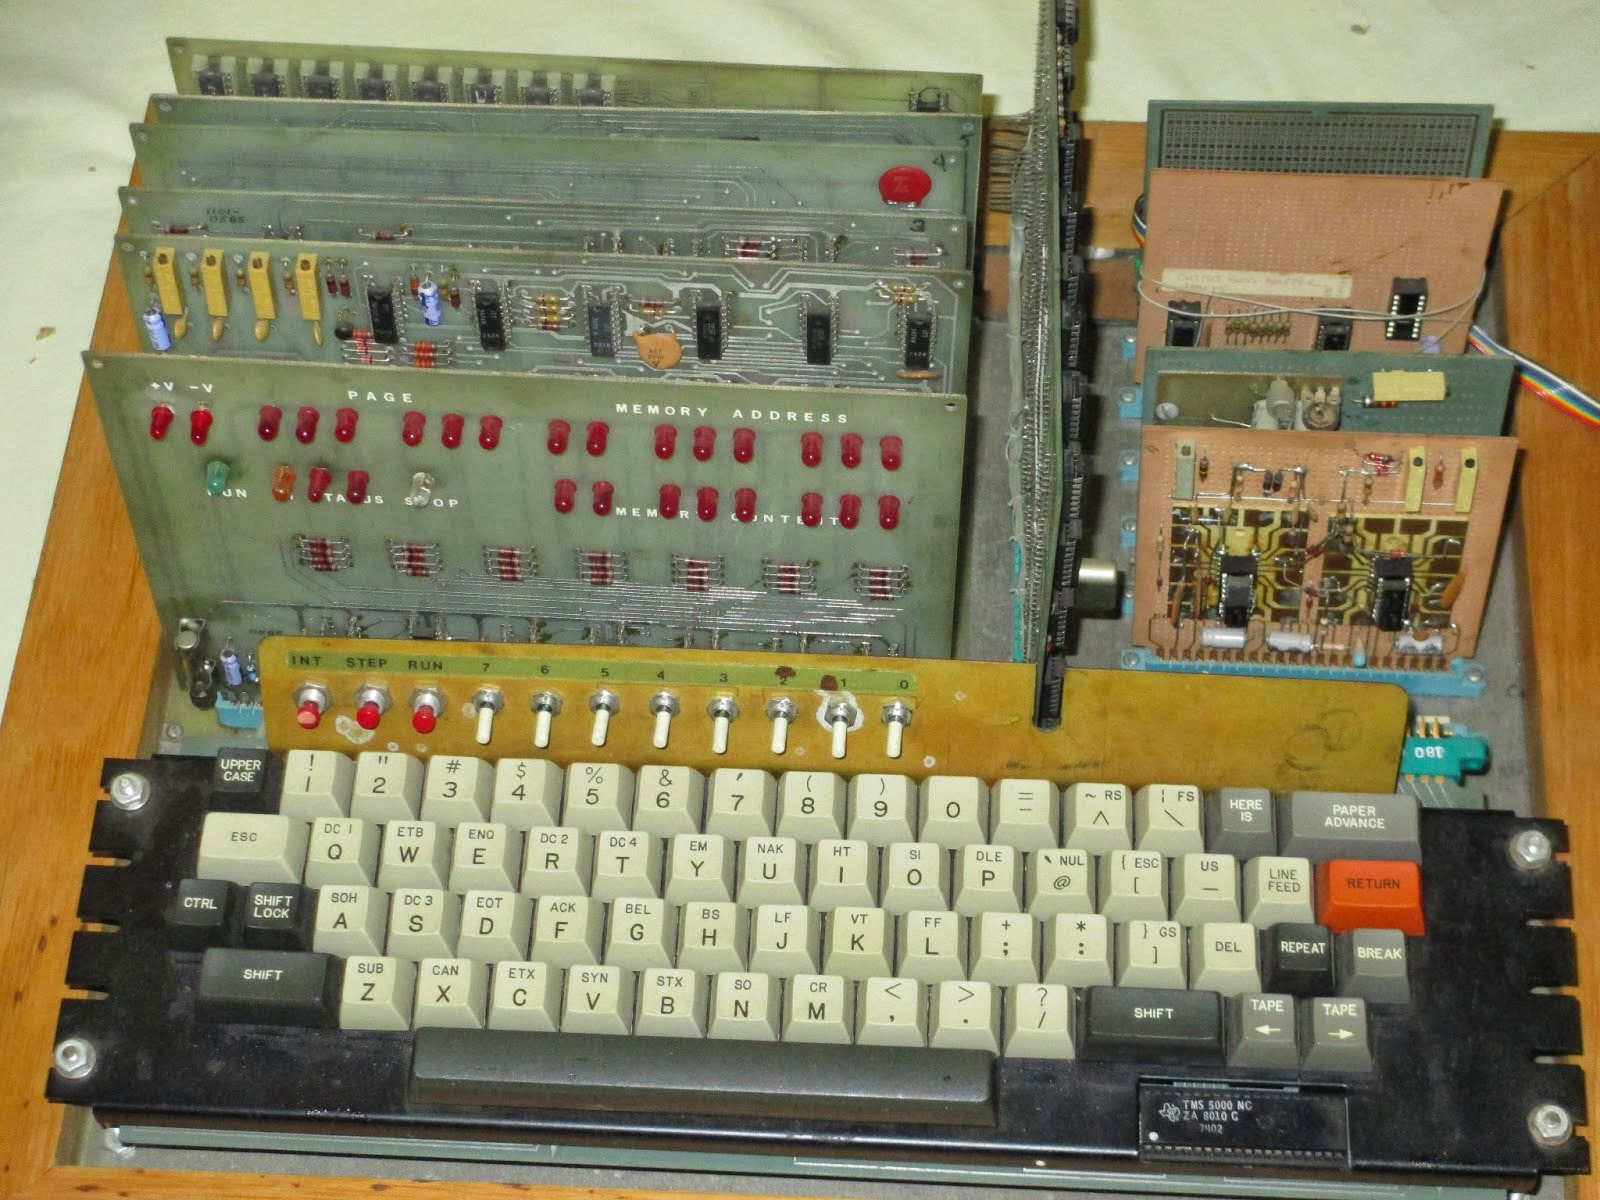
\includegraphics[width=.7\textwidth]{scelbi.jpg}
\caption{A "single board" computer}
\end{figure}
\end{frame}

\subsubsection{Pioneers}

\begin{frame}{SBC Pioneers}
\centering
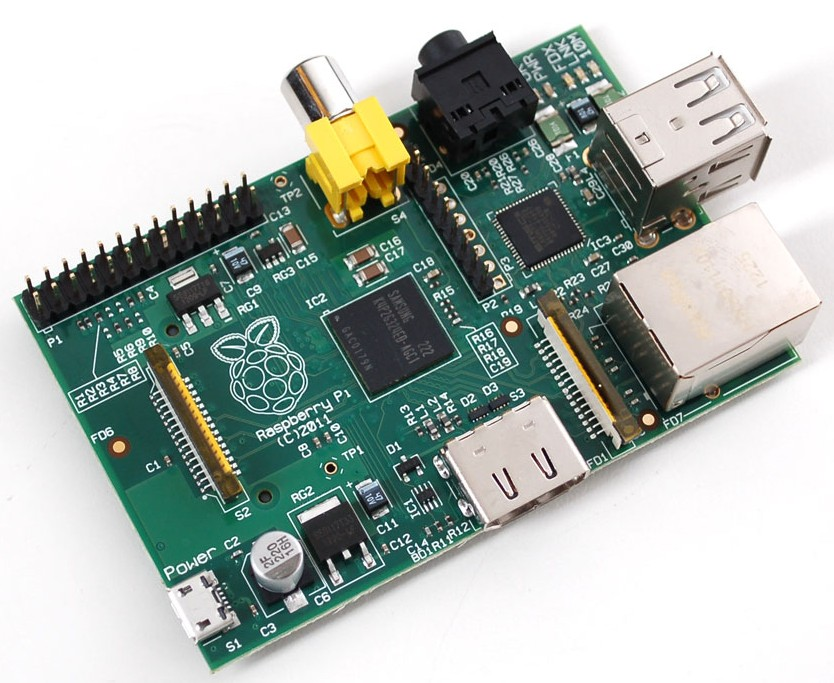
\includegraphics[width=.40\linewidth]{raspi.jpg}
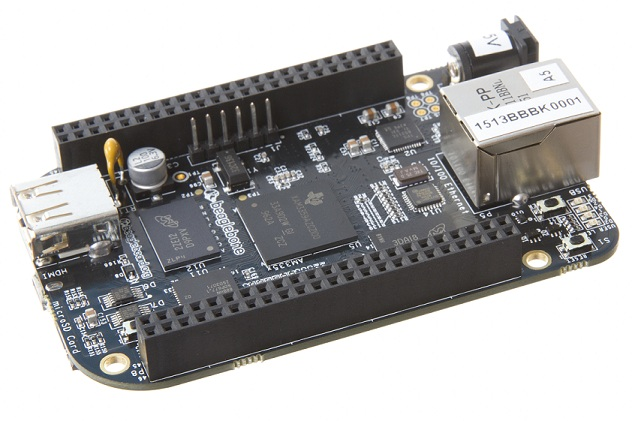
\includegraphics[width=.40\linewidth]{beagle.jpg}
\newline
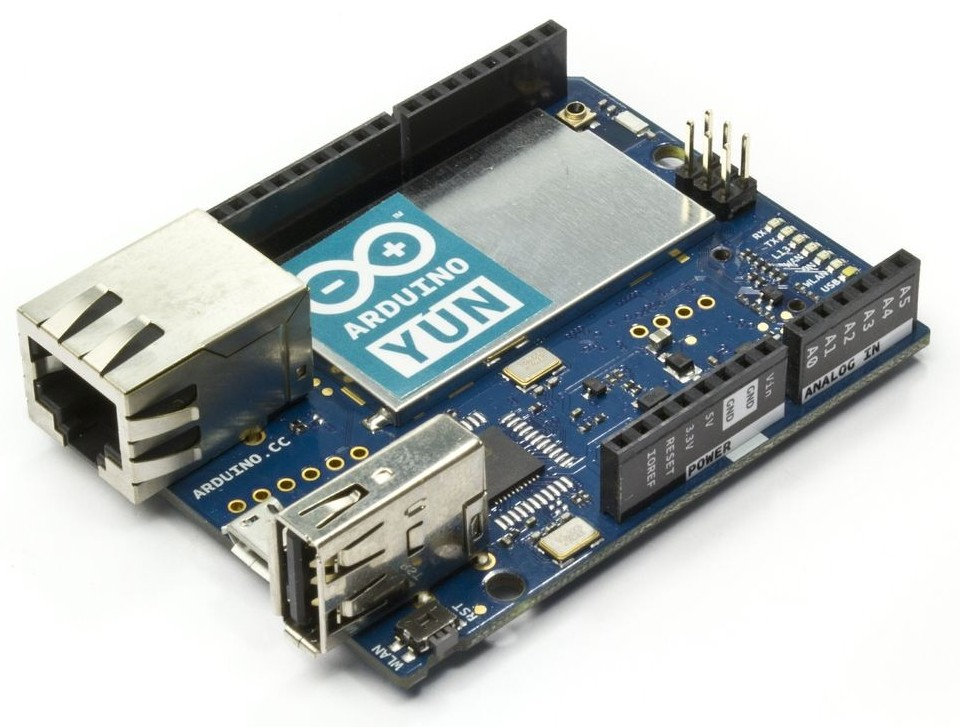
\includegraphics[width=.40\textwidth]{arduino-yun.jpg}
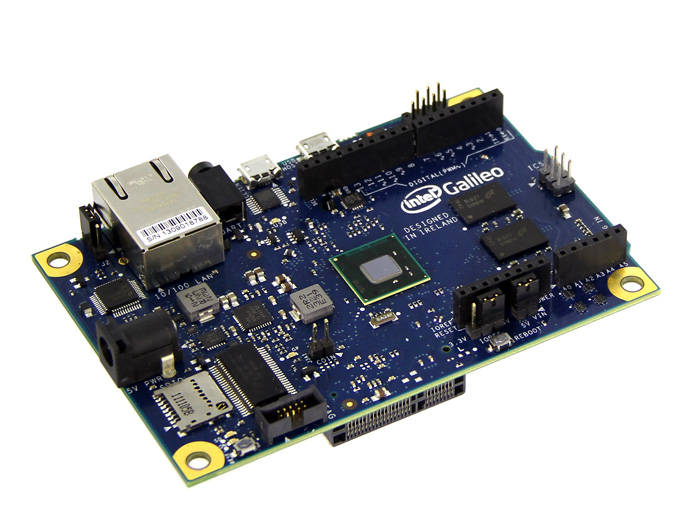
\includegraphics[width=.40\textwidth]{galileo.jpg}
\end{frame}


\subsubsection{Projects}

\begin{frame}{Why are SBC useful?}
\begin{figure}
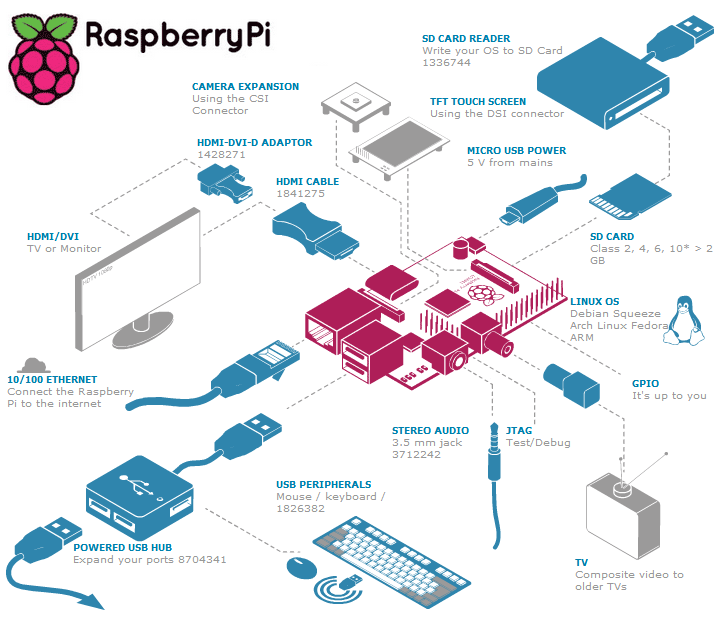
\includegraphics[width=.7\textwidth]{raspi-peripherals.png}
\caption{Raspberry Pi with a range of available peripherals}
\end{figure}
\end{frame}


\begin{frame}{Done by others}
	\begin{itemize}
	\item CNC and 	3D printer controllers
	\item Clusters, parallel computers	
	\item Handheld game devices
	\item Computer console emulators (MAME)
	\item Vending machine controllers
	\item Various robots
	\item Bitcoin miners
	\item Educational tools
	\end{itemize}
\end{frame}

\subsubsection{CHIP ?}

\begin{frame}{CHIP - 9 dollar computer}
	\begin{figure}
	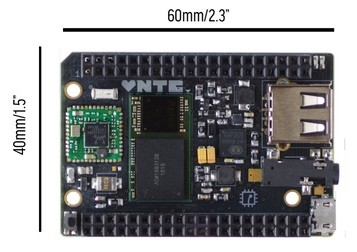
\includegraphics[width=.5\textwidth]{chip.jpg}
	\caption{Too good to be true?}
	\end{figure}
\end{frame}


%
%\subsection{Development}
%
%
%\begin{frame}{Development Boards}
%	asdf
%\end{frame}


\subsection{Embedded}

\begin{frame}{Embedded Computing}
	\begin{figure}
	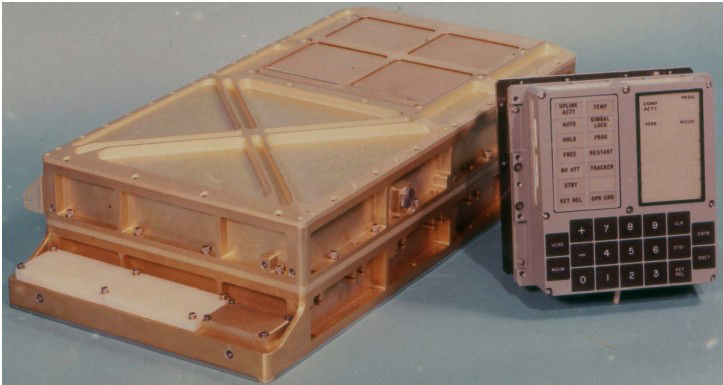
\includegraphics[width=.8\textwidth]{apollo-guidance.jpg}
	\caption{Apollo Guidance Computer and Numeric Display with a Keyboard}
	\end{figure}
\end{frame}



\begin{frame}{Embedded Confusion}
	\centering
	
	\begin{block}{Question} 
	Is Raspberry Pi an embedded system?
	\end{block}

	\vskip .7cm
	
\includegraphics[width=.20\textwidth]{raspi-logo.jpg}
	\hskip 3cm
	
\includegraphics[width=.20\textwidth]{arduino-logo.png}
	\vskip .7cm

	\begin{block}{Question} 
	Is Arduino an embedded module?
	\end{block}
\end{frame}

\subsubsection{Arduino}

\begin{frame}{Arduino vs Arduino}
	\begin{figure}
	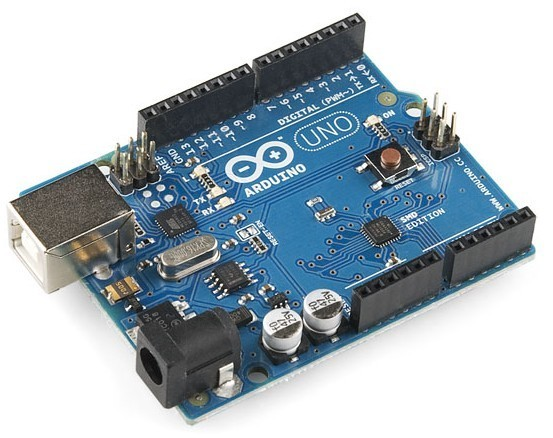
\includegraphics[width=.7\textwidth]{arduino-uno.jpg}
	\caption{The mighty Arduino Uno}
	\end{figure}
\end{frame}

\begin{frame}{Symbiosis of the Two}
	\begin{figure}
	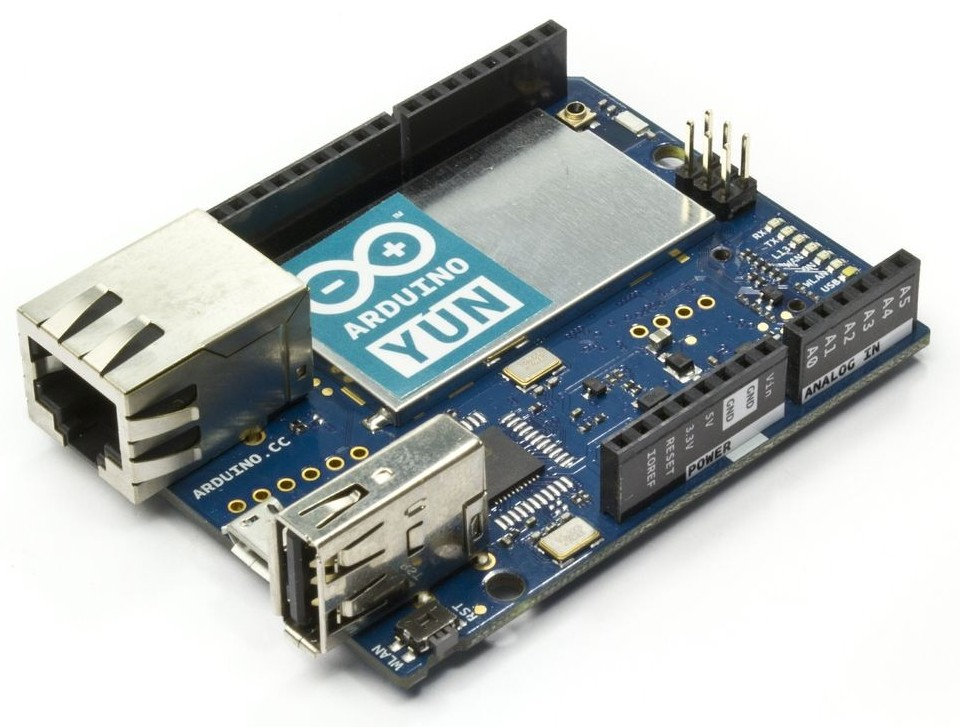
\includegraphics[width=.7\textwidth]{arduino-yun.jpg}
	\caption{Linux board + micro-controller = versatility}
	\end{figure}
\end{frame}


\subsubsection{Common Boards}

\begin{frame}{Cheap and Common Embedded Boards}
	\centering
	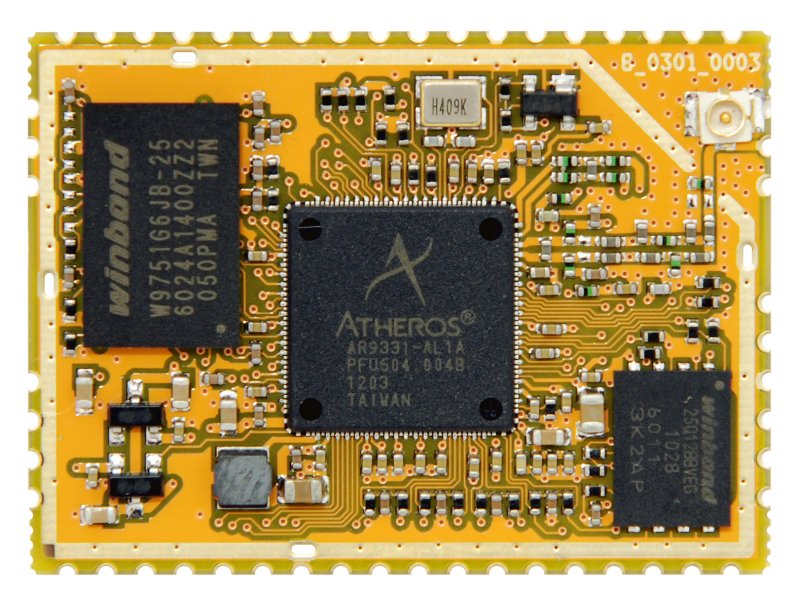
\includegraphics[width=.40\linewidth]{carambola2.png}
	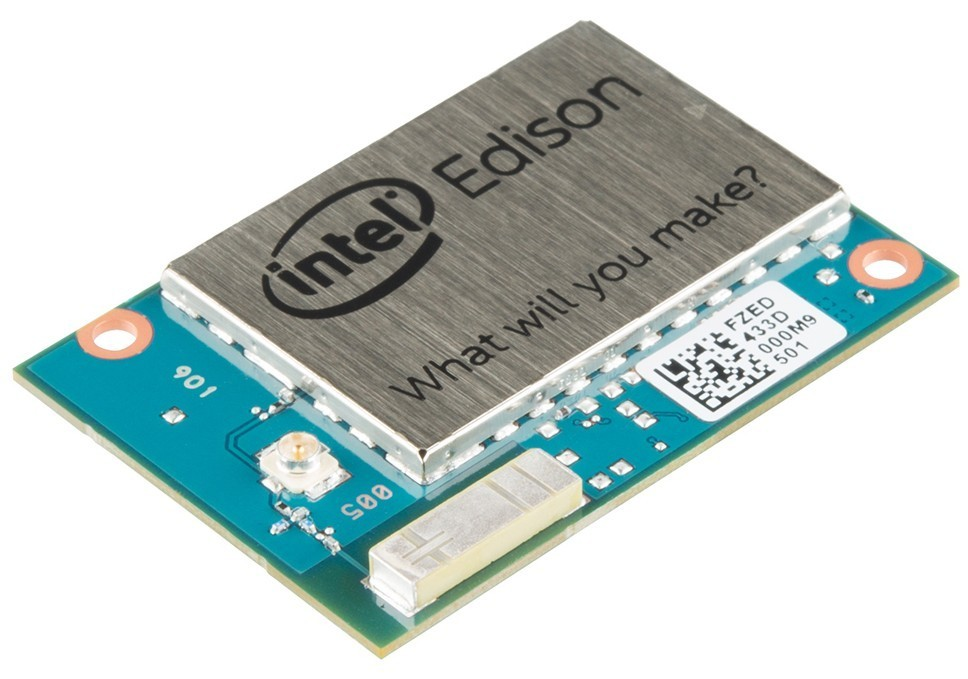
\includegraphics[width=.40\textwidth]{intel-edison.jpg}
	\vskip 1cm
	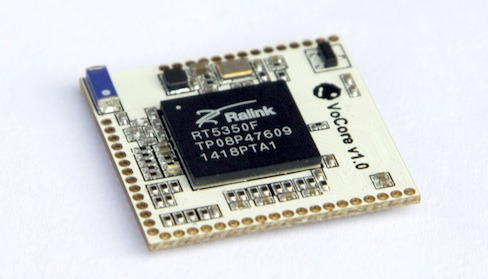
\includegraphics[width=.40\linewidth]{vocore.jpg}
	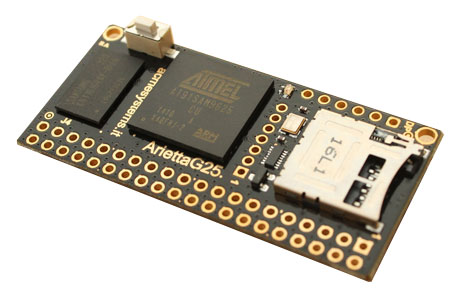
\includegraphics[width=.40\textwidth]{arietta-g25.jpg}
\end{frame}

\subsubsection{GL-Inet}

\begin{frame}{GL-Inet Smart Router}
	\begin{figure}
	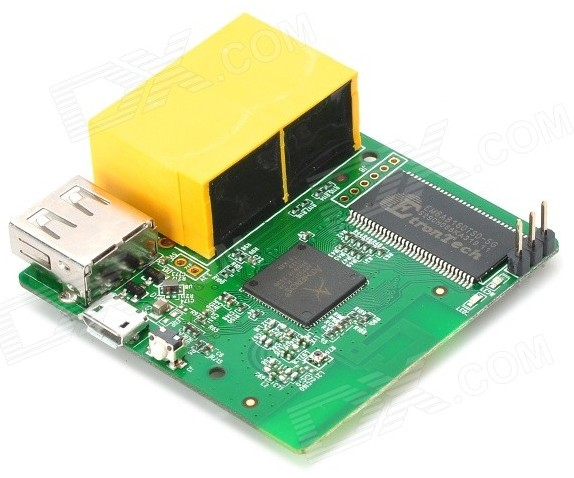
\includegraphics[width=.7\textwidth]{glinet.jpg}
	\caption{The personal pavorite number 1}
	\end{figure}
\end{frame}


\begin{frame}{TP-Link WR703n}
	\begin{figure}
	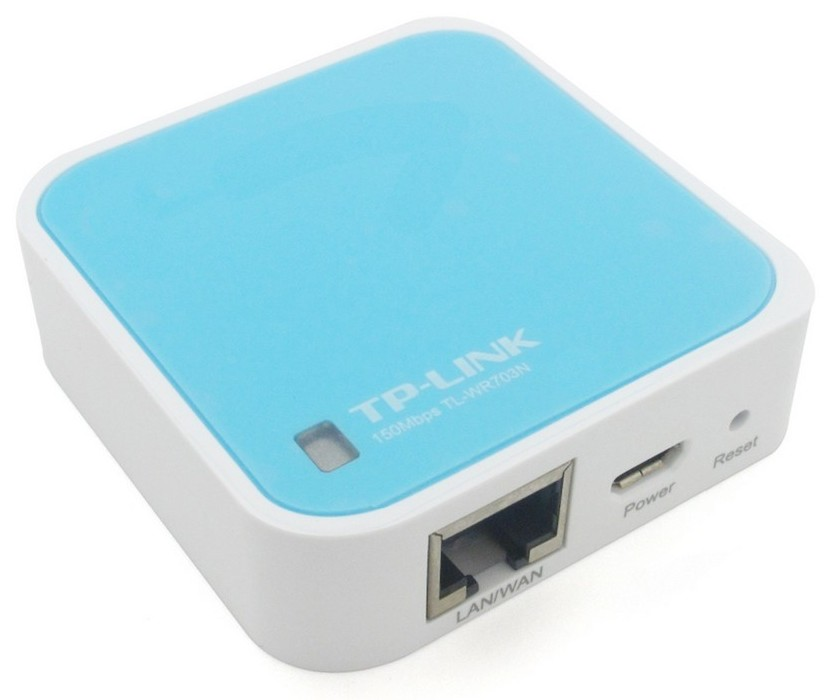
\includegraphics[width=.7\textwidth]{wr703n.jpg}
	\caption{The predecessor of a GL.Inet}
	\end{figure}
\end{frame}


\section{Opereating system}

\begin{frame}{Why Linux?}
	\begin{figure}
	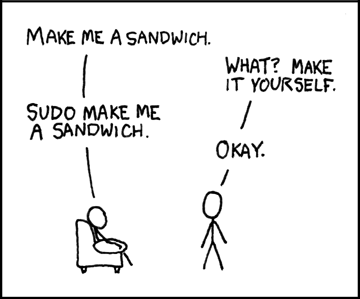
\includegraphics[width=.7\textwidth]{sandwich.png}
	\caption{Randall Munroe knew it before}
	\end{figure}
\end{frame}

\subsection{Linux}

\begin{frame}{The Linux Ecosystem}
	\begin{figure}
	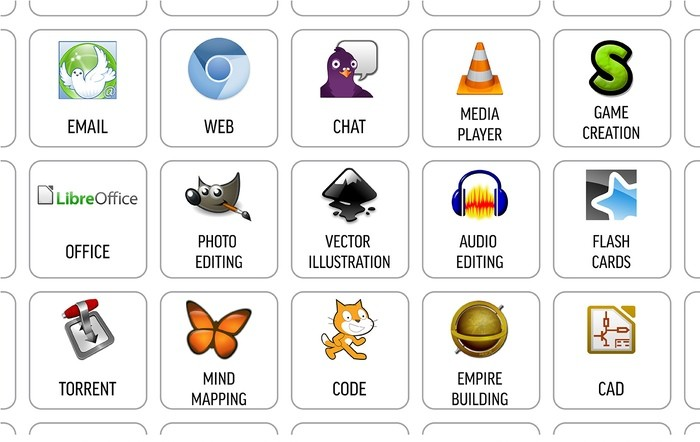
\includegraphics[width=.75\textwidth]{linux-apps.jpg}
	\caption{Marketing says: IT'S ALL FREE!}
	\end{figure}
\end{frame}

\subsection{OpenWRT}

\begin{frame}{OpenWRT}
	\centering
	
	\begin{block}{Question}
	What can you do with a full blown Linux, given only 16MB, 8MB or even 4MB RAM or Flash is available?
	\end{block}
	
	\vskip .4cm
	\begin{figure}
	
\includegraphics[width=.4\textwidth]{busybox.png}
	\caption{BusyBox (+ uClibc)}
	\end{figure}	

\end{frame}



\section{The Future}


\begin{frame}{Where is it all going?}
	\begin{figure}
	
\includegraphics[width=.4\textwidth]{hacked.png}
%	\caption{Security or Privacy, anyone?}
	\end{figure}
\end{frame}

\subsection{Samsung ARTIK}


\begin{frame}{Samsung ARTIK boards}
	\begin{figure}
	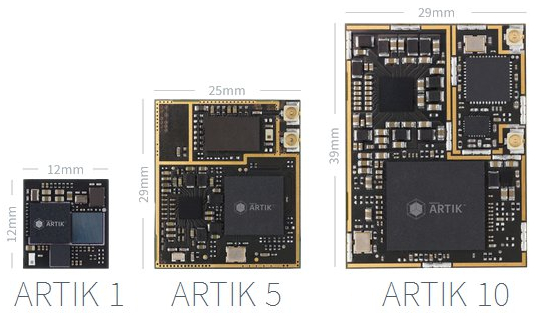
\includegraphics[width=.8\textwidth]{samsung-artik.jpg}
	\caption{Can you (crypto)secure my computing?}
	\end{figure}
\end{frame}

\begin{frame}{ARTIK TrustZone}
	\begin{quote}
	The secure element supports ARM TrustZone, and is supported with a machine learning based anomaly detection system that helps identify abnormalities and unusual behavior that may reflect hacking or intrusion activity, says \textbf{Samsung}.
	\end{quote}

%	\begin{figure}
%	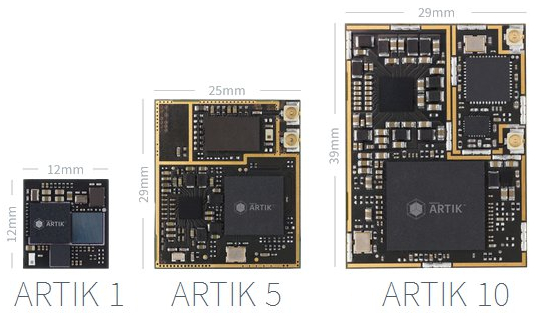
\includegraphics[width=.8\textwidth]{samsung-artik.jpg}
%	\caption{Secure Element, TEE Trust Zone}
%	\end{figure}
\end{frame}

\subsection{IoT}

\begin{frame}{Internet of Things}
	\begin{block}{Definition}
	A network of physical objects or “things” embedded with electronics, software, sensors and connectivity to enable it to achieve greater value and service by \textbf{exchanging data with the manufacturer}, operator and/or other connected devices.
	\end{block}
\end{frame}

\subsubsection{Intel}

\begin{frame}{Intel's part of the IoT story}
	\begin{figure}
	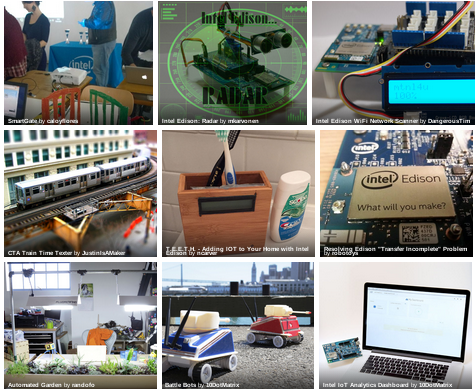
\includegraphics[width=.7\textwidth]{intel-iot.png}
	\caption{The dedicated Instructables.com Intel IoT page}
	\end{figure}
\end{frame}

\section{Epilogue}

\begin{frame}{Epilogue}
	\centering
	{\large Thank you $\cdot$ !`Gracias! $\cdot$ Ďakujem}
	
	\vskip 2cm
	Peter Babič	$@$peter\_babic

\end{frame}


%\begin{frame}
%	\printbibliography
%\end{frame}

\end{document}



%\begin{figure}
%	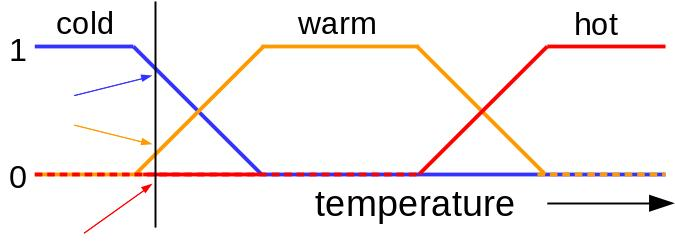
\includegraphics[width=.75\textwidth]{fuzzy-set.jpg}
%	\caption{Example interpretation of fuzzy sets. At the given temperature point, we can tell that the measured medium is "not hot", "slightly warm" and "almost cold".
%	\label{fig:fuzzy-set}}
%\end{figure}


%\begin{itemize}
%\item Use \texttt{tabular} for Basic Tables! --- See Table~\ref{tab:widgets}, for Example.
%\item You Can Upload a Figure (JPEG, PNG or PDF) Using the Files Menu. 
%\item to Include It in Your Document, Use the \texttt{includegraphics} Command (See the Comment Below in the Source Code).
%\end{itemize}


%\begin{table}
%\centering
%\begin{tabular}{l|r}
%Item & Quantity \\\hline
%Widgets & 42 \\
%Gadgets & 13
%\end{tabular}
%\caption{\label{tab:widgets}An example table.}
%\end{table}


%  Let $X_1, X_2, \ldots, X_n$ be a sequence of independent and identically distributed random variables with $\text{E}[X_i] = \mu$ and $\text{Var}[X_i] = \sigma^2 < \infty$, and let
%  $$S_n = \frac{X_1 + X_2 + \cdots + X_n}{n}
%  = \frac{1}{n}\sum_{i}^{n} X_i$$
%  denote their mean. Then as $n$ approaches infinity, the random variables $\sqrt{n}(S_n - \mu)$ converge in distribution to a normal $\mathcal{N}(0, \sigma^2)$.


% \vskip 1cm

% \begin{block}{Examples}
% Some examples of commonly used commands and features are included, to help you get started.
% \end{block}
